\documentclass[aspectratio=1610]{beamer}
%\documentclass[aspectratio=1610, handout]{beamer}
\usepackage[utf8]{inputenc}
\usepackage{ragged2e}
\usepackage{xcolor}
\usepackage[italian]{babel}
\usepackage{multirow}
\usetheme[progressbar=frametitle,titleformat=smallcaps]{metropolis}
\setbeamertemplate{frame numbering}[fraction]
\setbeamercovered{dynamic}
\definecolor{rosso}{RGB}{255, 0, 0}
\definecolor{giallo}{RGB}{254,212,23}
\hypersetup{colorlinks=true,linkcolor=black,urlcolor=rosso}
\setbeamercolor{palette primary}{fg=black, bg=giallo}
\setbeamercolor{background canvas}{bg=white}
\setbeamercolor{normal text}{fg=black}
\setbeamercolor{progress bar}{fg=rosso}
\setbeamercolor{framesubtitle}{fg=rosso}
\setbeamercolor{normal text .dimmed}{fg=giallo}
\setbeamercolor{block title alerted}{fg=rosso, bg=giallo}
\setbeamerfont{caption}{size=\tiny}
\setbeamerfont{caption name}{size=\tiny}
\setlength{\abovecaptionskip}{0pt}
\makeatletter
\metroset{block=fill}
\setlength{\metropolis@progressinheadfoot@linewidth}{1pt} 
\setlength{\metropolis@progressonsectionpage@linewidth}{1pt}
\setlength{\metropolis@titleseparator@linewidth}{1pt}
\makeatother

\title{GESTORE DELLE PERIFERICHE}
\subtitle{3° livello del Sistema Operativo}
\date{}
\institute{\textit{
        Fonti:
        \begin{itemize}
            \item[-] \href{https://www.unimi.it/it/corsi/laurea-triennale/informatica}{Appunti Università degli Studi di Milano}
        \end{itemize}
    }
}

\begin{document}

\begin{frame}[plain, noframenumbering]
    \titlepage
\end{frame}

\section{PERIFERICHE}

\begin{frame}{PERIFERICHE E DRIVER}
    \begin{columns}
        \column{.5\textwidth}
        \begin{itemize}
            \item \textbf{INPUT}
            \item \textbf{OUTPUT}
            \item \textbf{INPUT/OUTPUT (I/O)}
        \end{itemize}
        \bigskip
        \tiny{\textbf{DRIVERS}}\\
        \tiny{\href{https://learn.microsoft.com/it-it/windows-hardware/drivers/gettingstarted/what-is-a-driver-}{Che cos'è un \textbf{DRIVER}?}}
        \column{.5\textwidth}
        \begin{figure}
            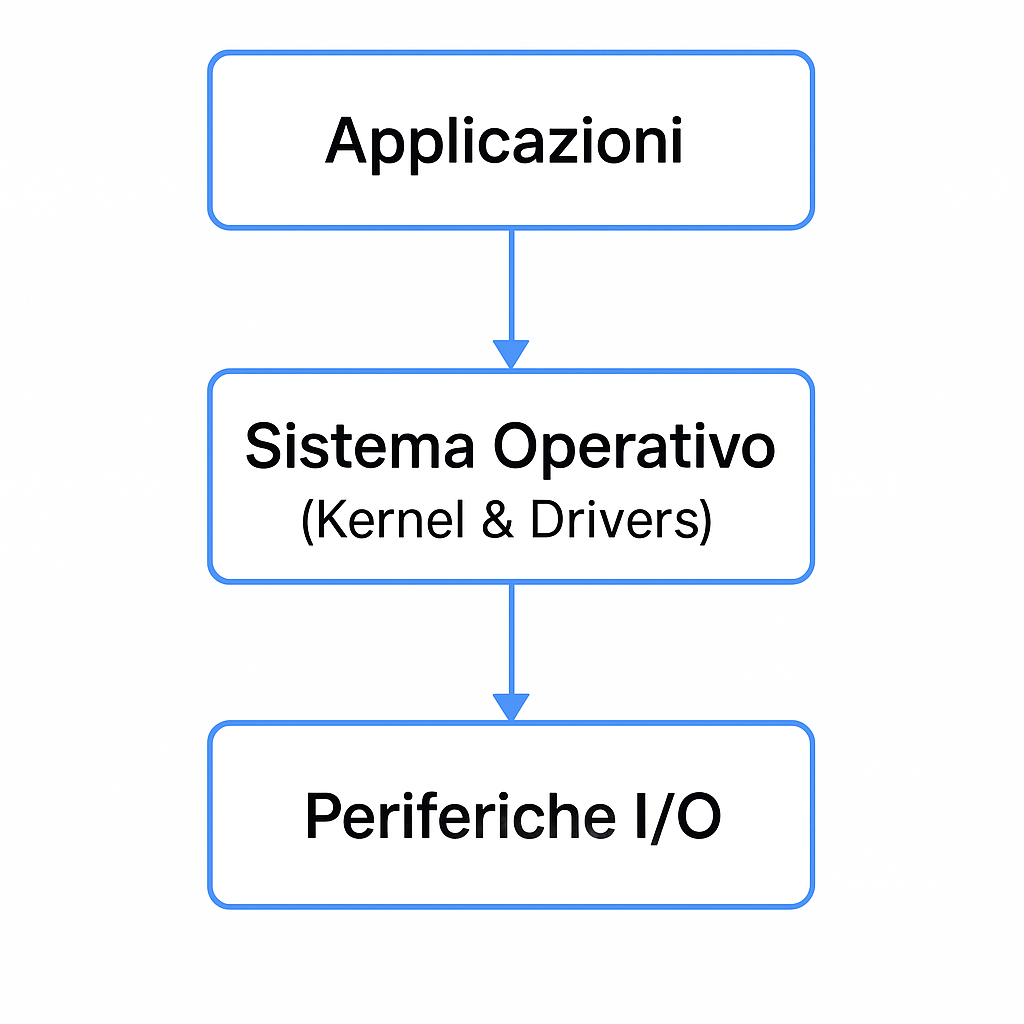
\includegraphics[width=\linewidth]{img/drivers.png}
            \caption{{creata con \href{https://chatgpt.com/}{ChatGPT}}}
        \end{figure}
    \end{columns}
\end{frame}

\section{TIPOLOGIE DI COMUNICAZIONE}

\begin{frame}{CONTINUOUS POLLING}
    \begin{alertblock}{DEFINIZIONE}
        \begin{minipage}{0.98\linewidth}
            \justifying
            CPU e periferica comunicano tramite un registro che contiene un parametro di stato (\textbf{bit di busy}) 
            che indica se la periferica è pronta a ricevere o inviare dati.
            \begin{itemize}
                \item 0: periferica libera;
                \item 1: periferica occupata.
            \end{itemize}
            Il sistema operativo deve continuamente interrogare la periferica (\textbf{busy wainting}) per sapere se è 
            libera o occupata. Non è un metodo efficiente, in quanto la CPU è costantemente occupata a 
            controllare lo stato della periferica e non può svolgere altre operazioni.\\
            \bigskip
            \tiny{\textbf{PERIODIC POLLING}}\\
            \tiny{\href{https://pollingratetest.org/}{Polling Rate Test}}
        \end{minipage}
    \end{alertblock}
\end{frame}

\begin{frame}{INTERRUPT}
    \begin{alertblock}{DEFINIZIONE}
        \begin{minipage}{0.98\linewidth}
            \justifying
            CPU e periferica comunicano tramite un \textbf{circuito fisico di Interrupt}. 
            Nel momento in cui la periferica è pronta a inviare dati, invia un segnale di interrupt alla CPU, 
            che interrompe l'esecuzione del processo corrente e inizia a eseguire il driver associato alla periferica. 
            La CPU può quindi eseguire altre operazioni mentre la periferica è occupata.\\ 
            La periferica può invece utilizzare una tipologia di comunicazione in continuous polling in attesa di 
            ricevere istruzioni da parte della CPU.
        \end{minipage}
    \end{alertblock}
\end{frame}

\section{ESEMPIO}

\begin{frame}{ESEMPIO}
    \only<1 | handout:1>{\begin{figure}
        
\includegraphics[width=\linewidth]{img/1.png}
        \caption{{creata con \href{https://www.canva.com/}{Canva}}}
    \end{figure}}
    \only<2 | handout:2>{\begin{figure}
        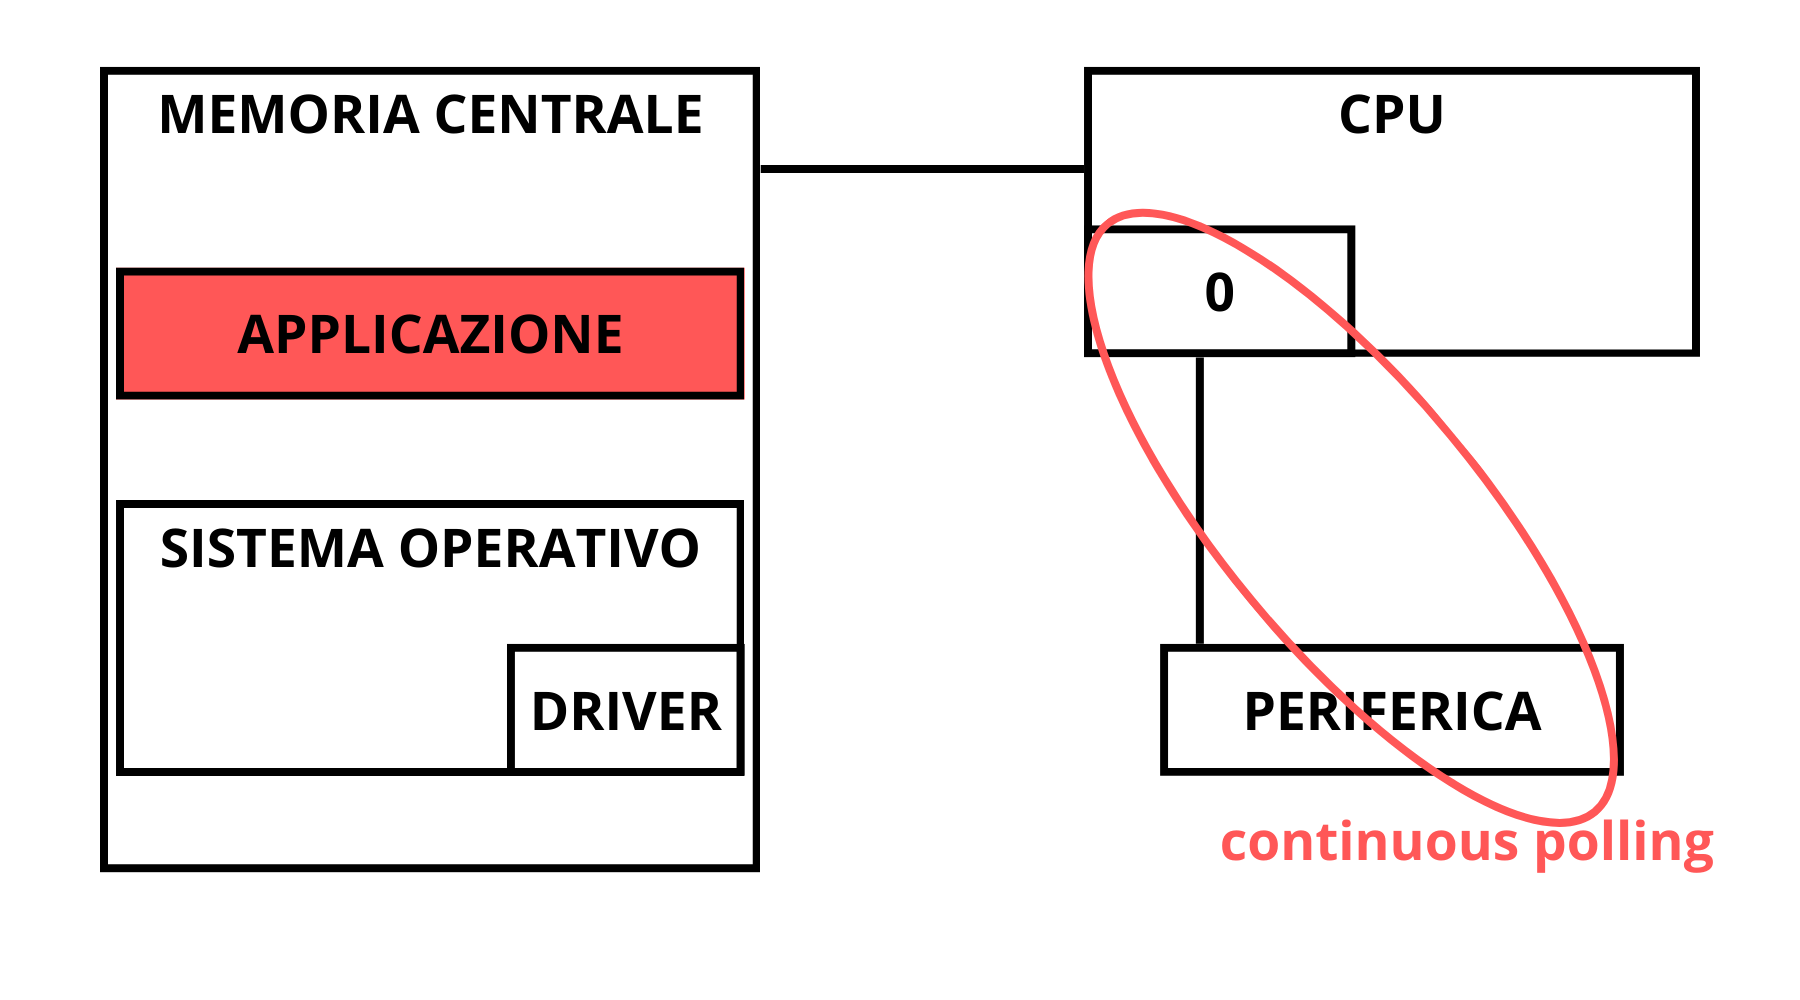
\includegraphics[width=\linewidth]{img/2.png}
        \caption{{creata con \href{https://www.canva.com/}{Canva}}}
    \end{figure}}
    \only<3 | handout:3>{\begin{figure}
        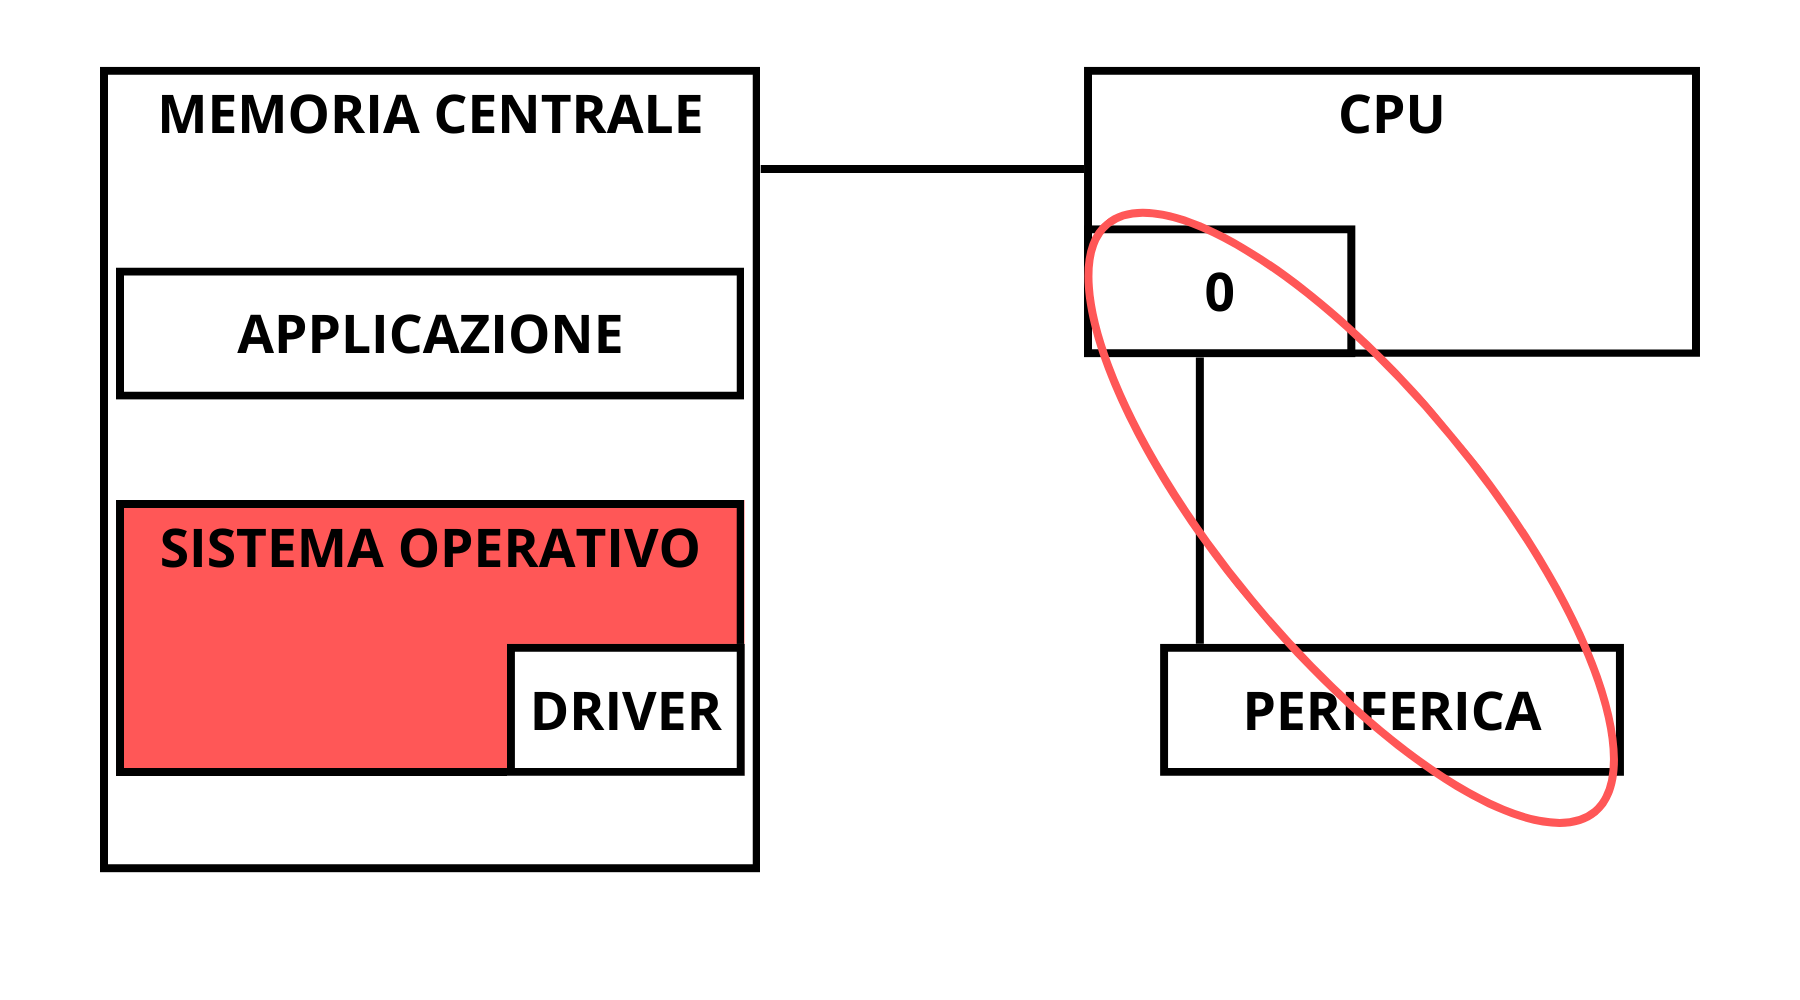
\includegraphics[width=\linewidth]{img/3.png}
        \caption{{creata con \href{https://www.canva.com/}{Canva}}}
    \end{figure}}
    \only<4 | handout:4>{\begin{figure}
        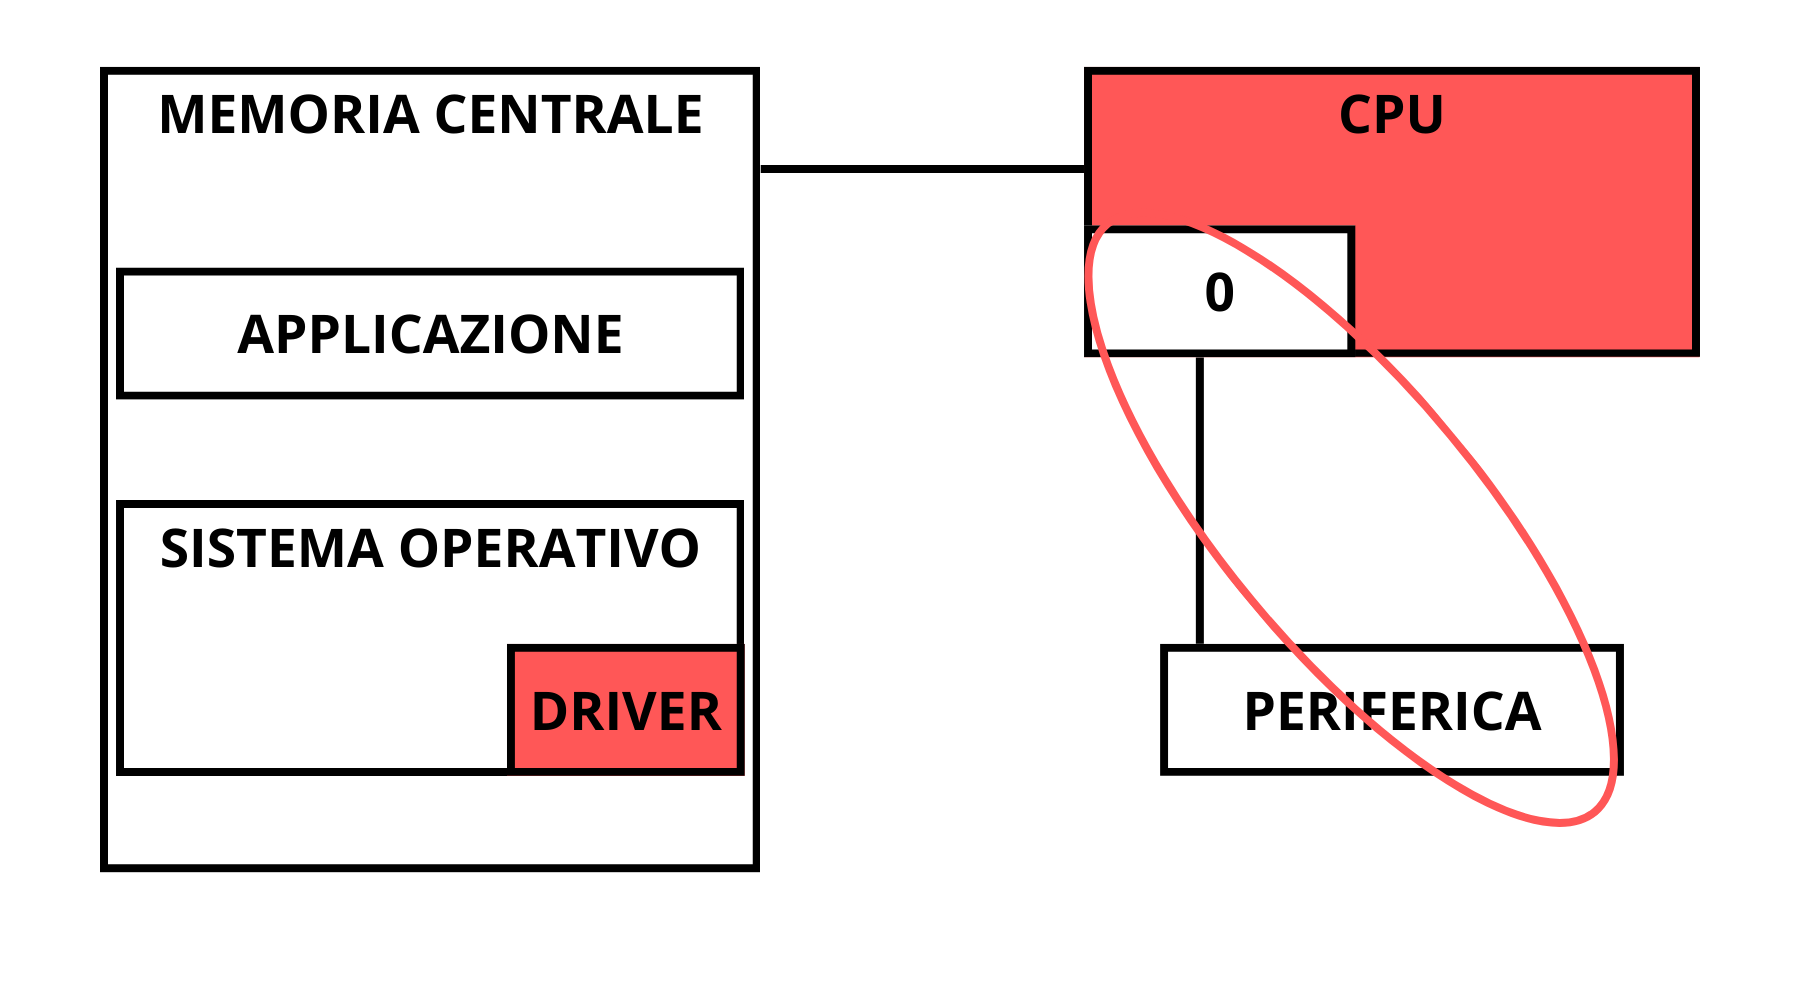
\includegraphics[width=\linewidth]{img/4.png}
        \caption{{creata con \href{https://www.canva.com/}{Canva}}}
    \end{figure}}
    \only<5 | handout:5>{\begin{figure}
        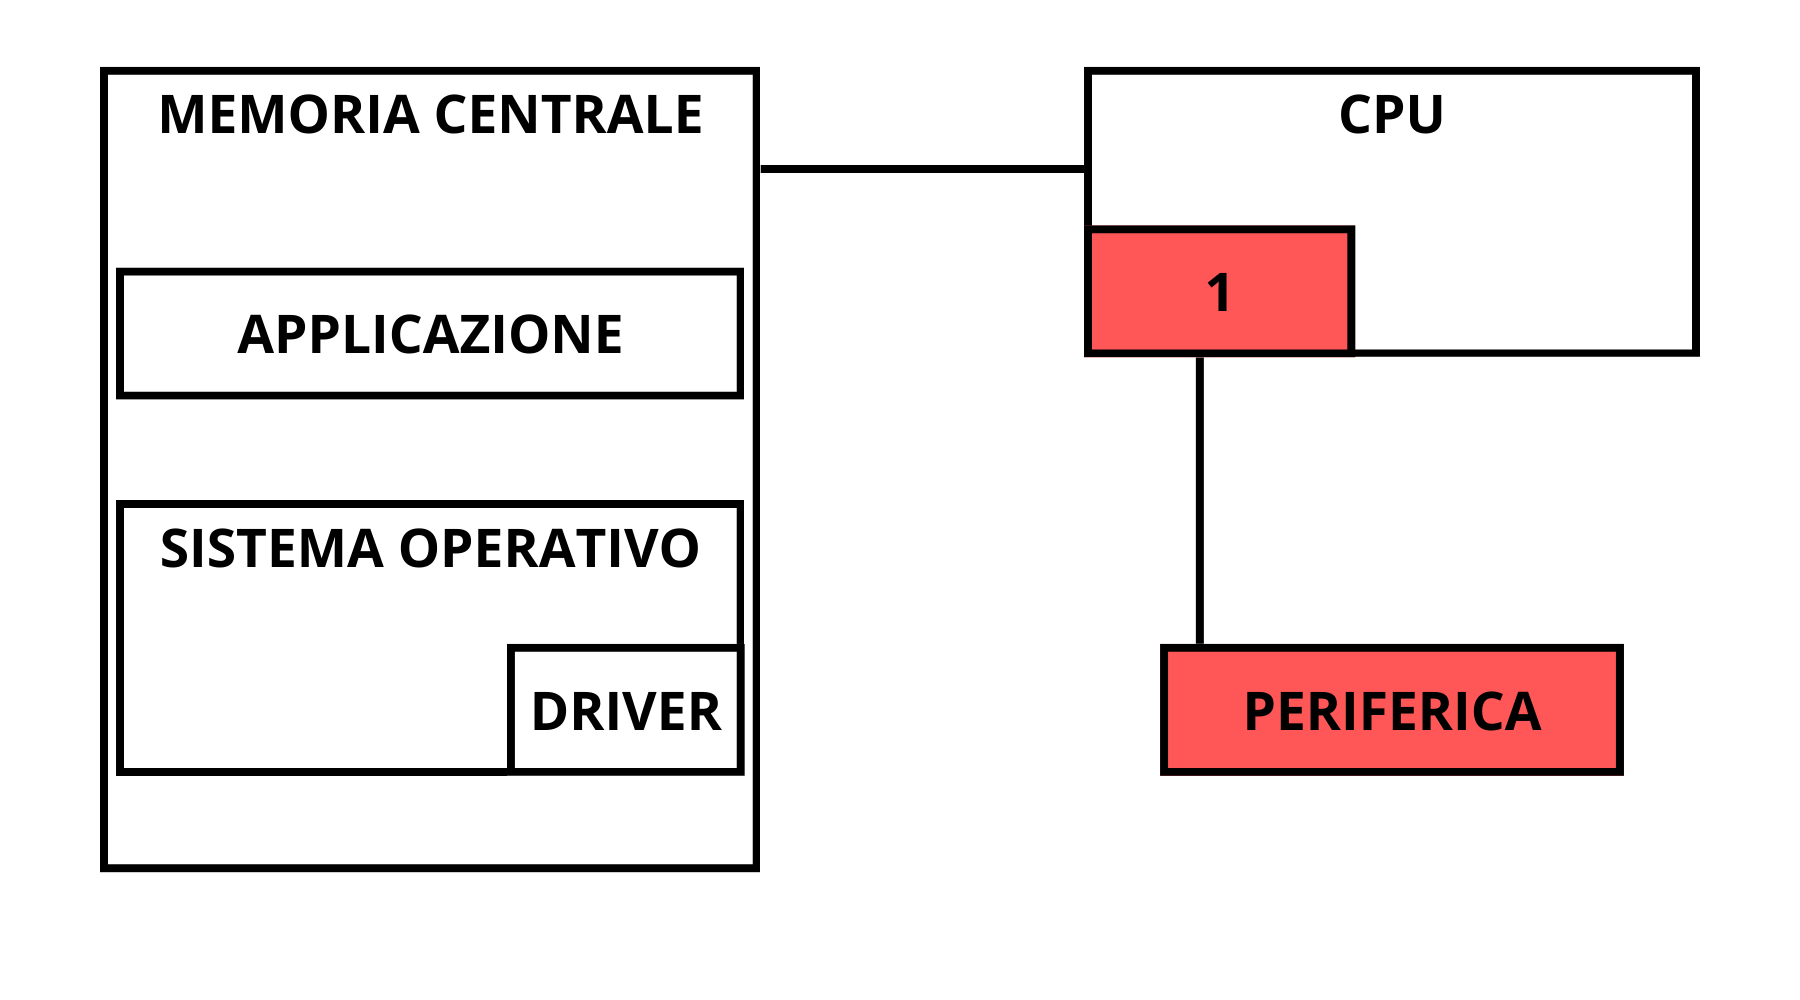
\includegraphics[width=\linewidth]{img/5.png}
        \caption{{creata con \href{https://www.canva.com/}{Canva}}}
    \end{figure}}
    \only<6 | handout:6>{\begin{figure}
        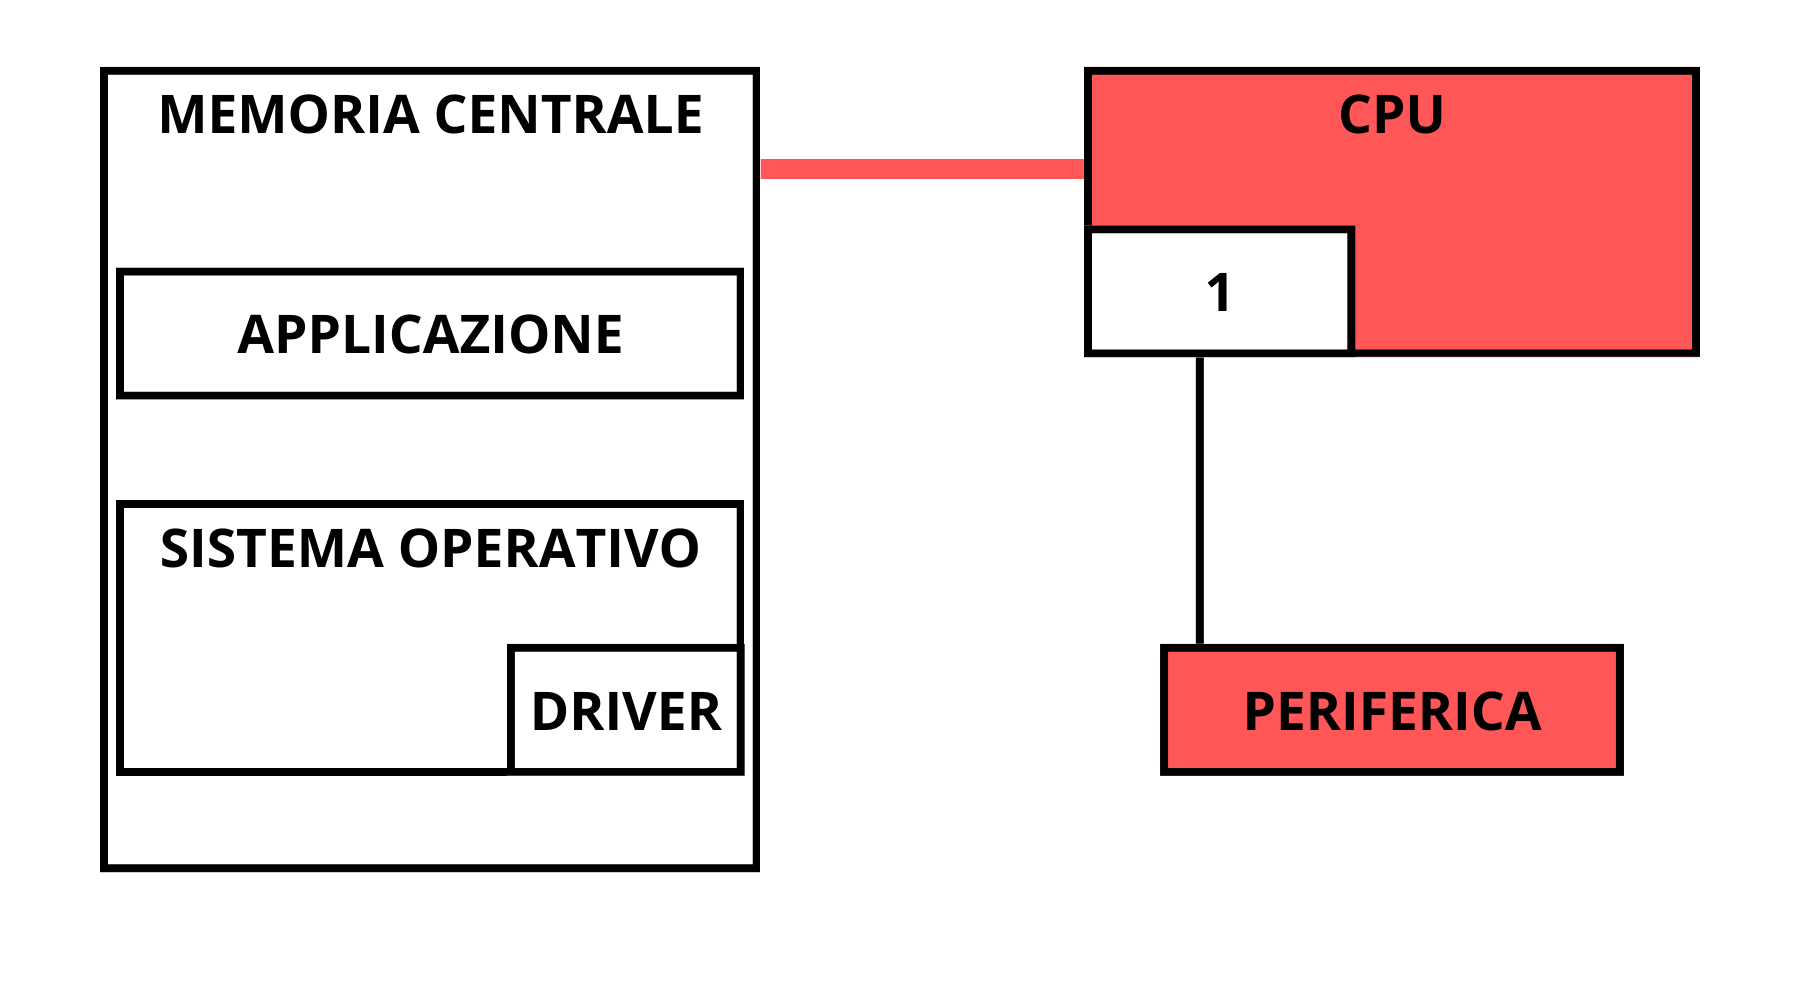
\includegraphics[width=\linewidth]{img/6.png}
        \caption{{creata con \href{https://www.canva.com/}{Canva}}}
    \end{figure}}
    \only<7 | handout:7>{\begin{figure}
        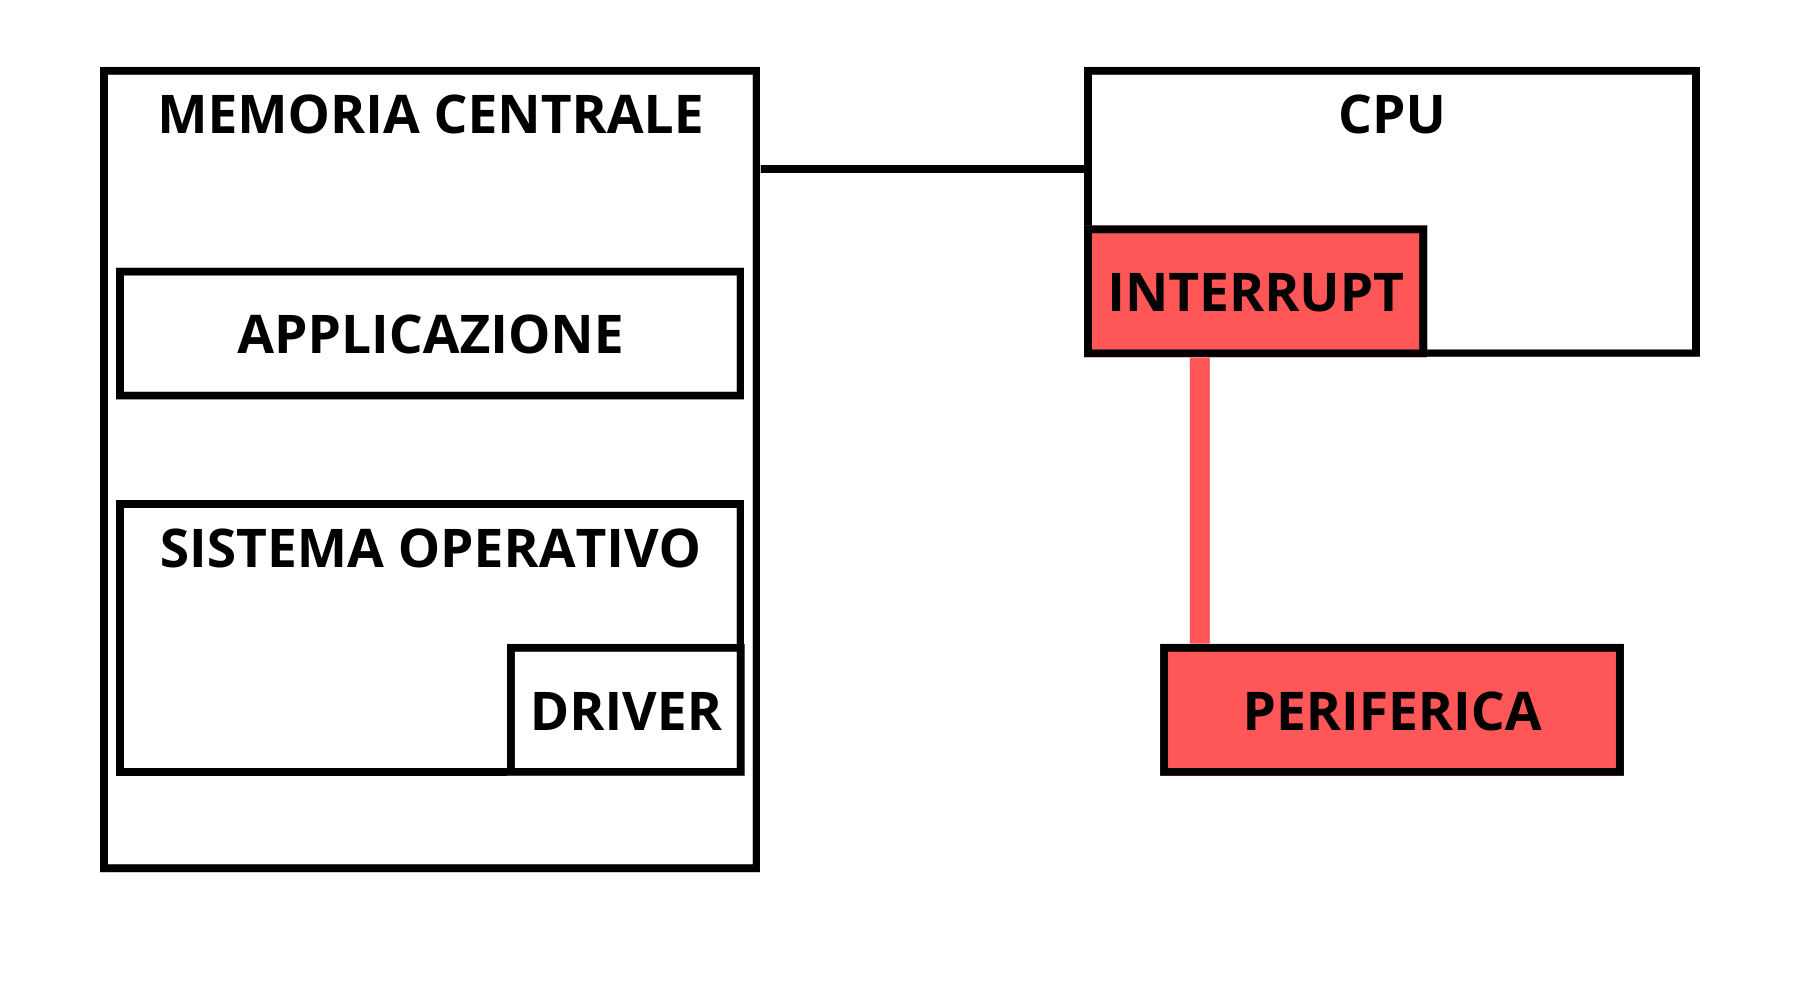
\includegraphics[width=\linewidth]{img/7.png}
        \caption{{creata con \href{https://www.canva.com/}{Canva}}}
    \end{figure}}
    \only<8 | handout:8>{\begin{figure}
        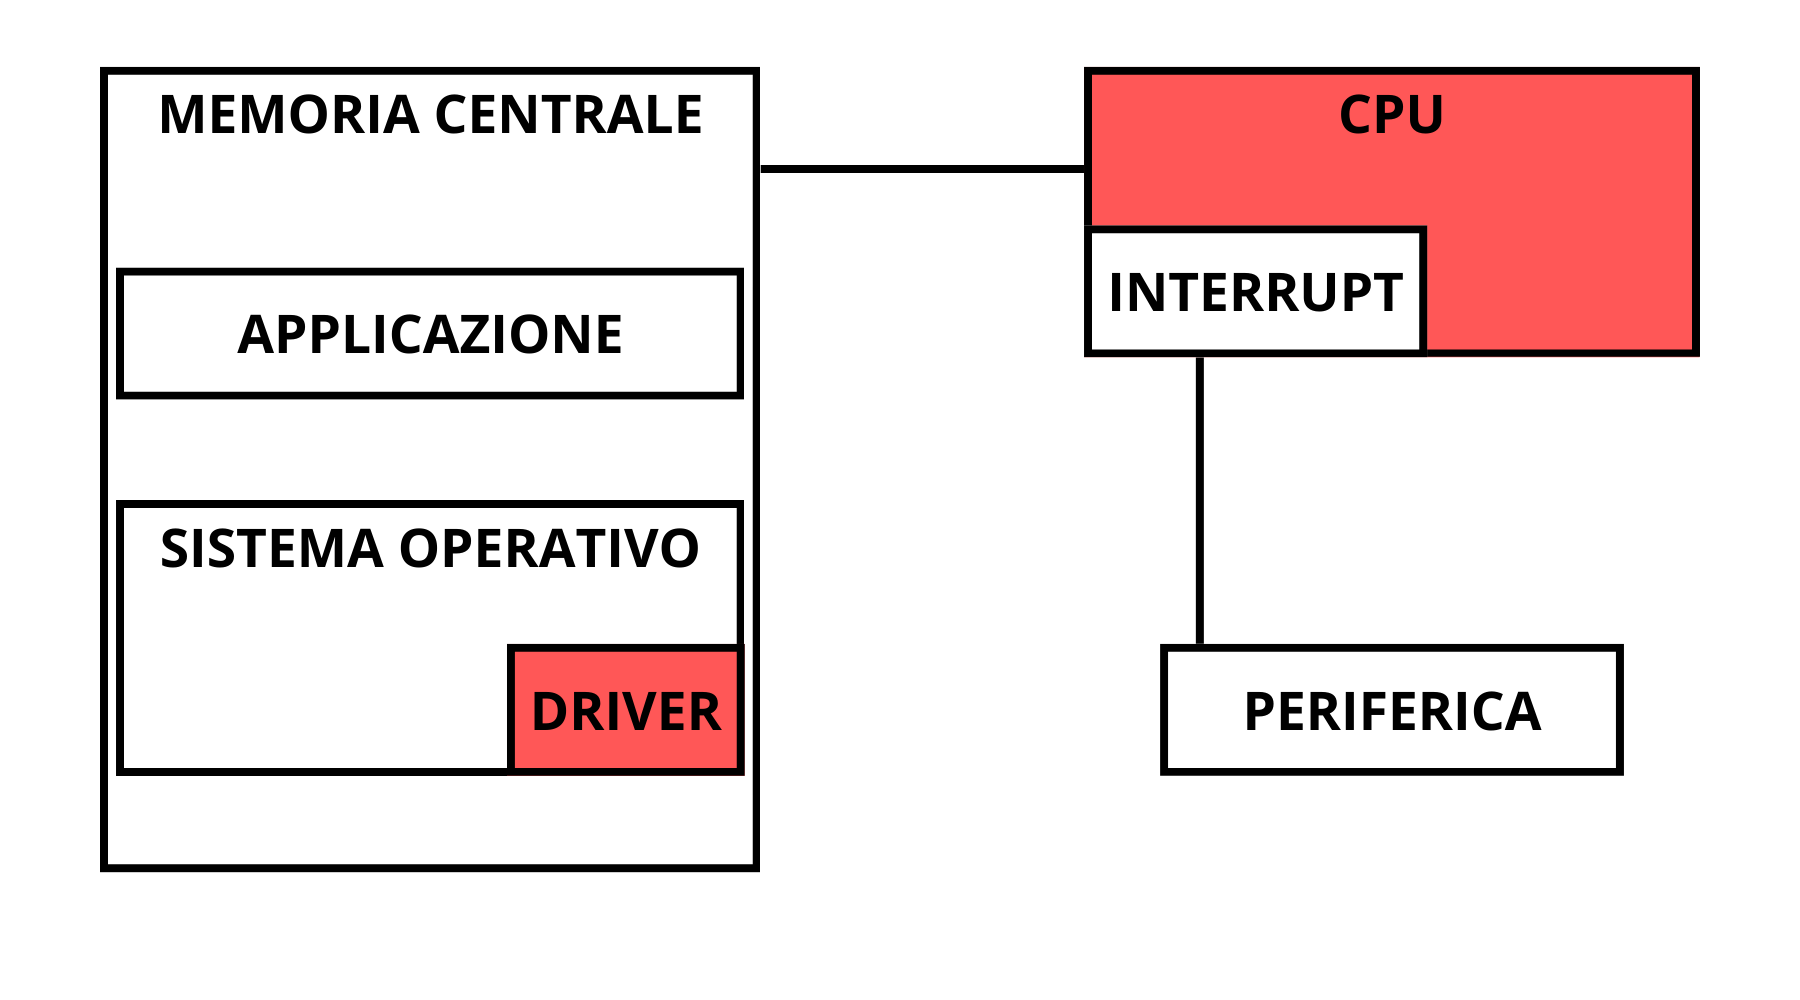
\includegraphics[width=\linewidth]{img/8.png}
        \caption{{creata con \href{https://www.canva.com/}{Canva}}}
    \end{figure}}
    \only<9 | handout:9>{\begin{figure}
        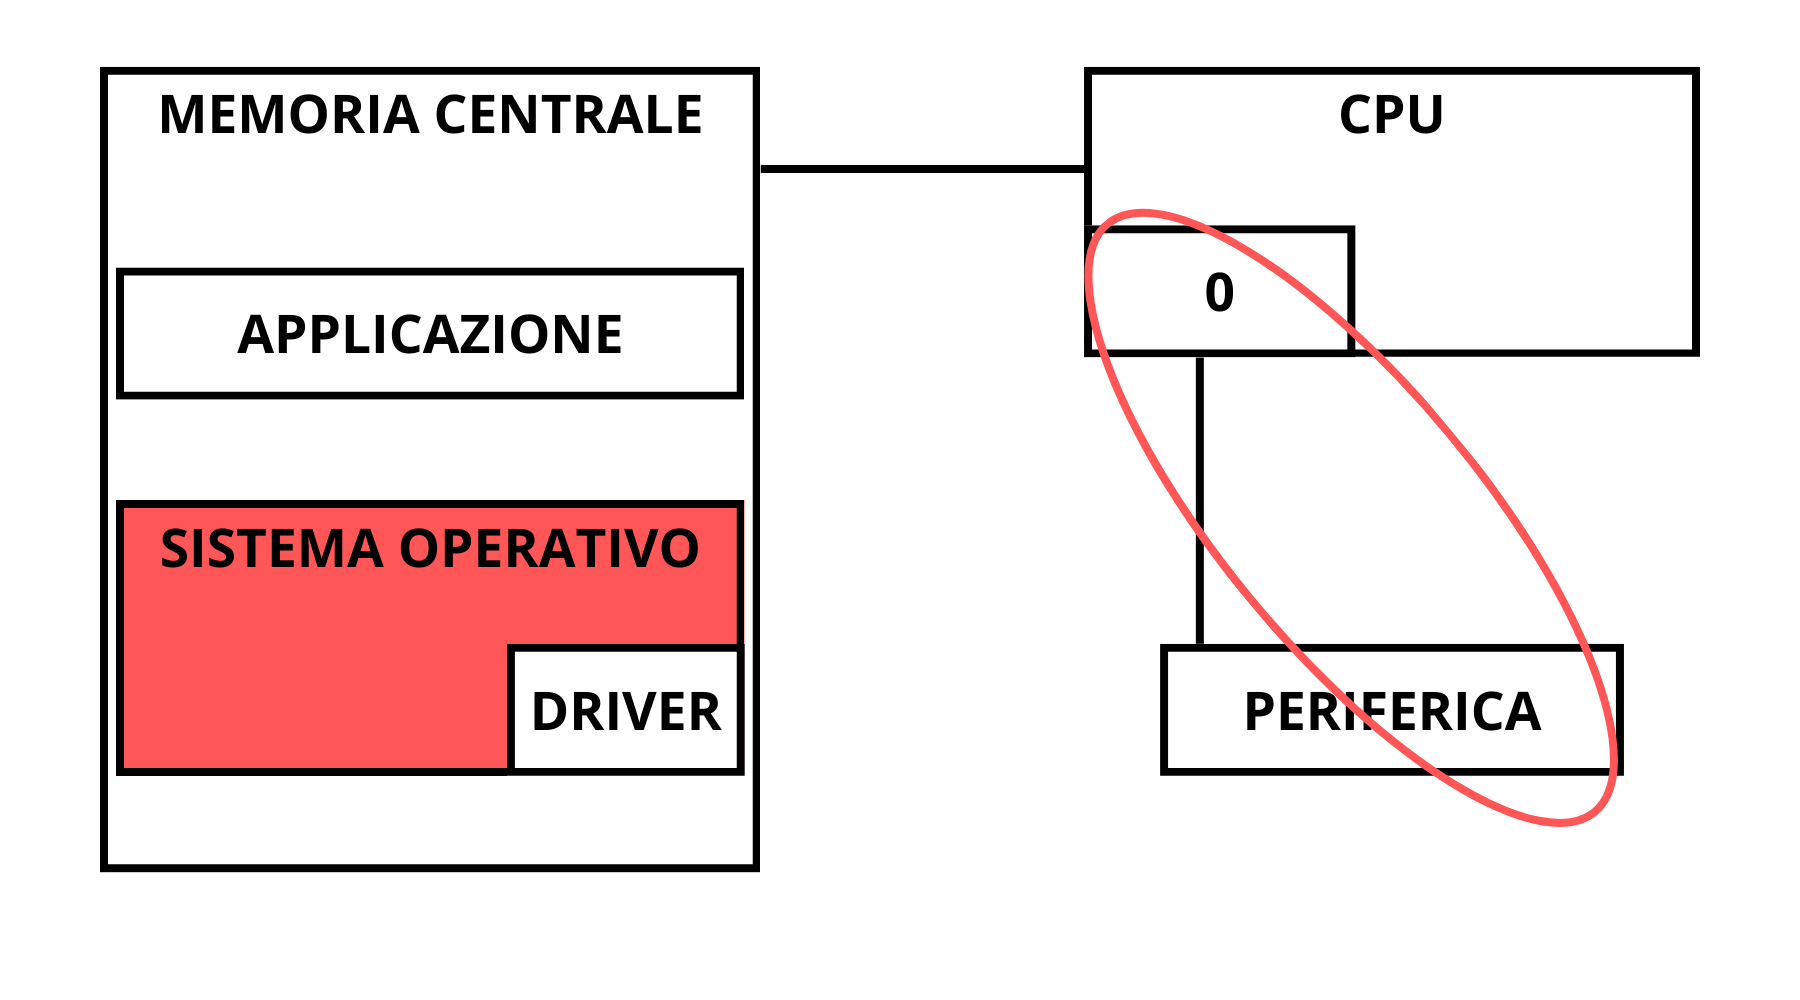
\includegraphics[width=\linewidth]{img/9.png}
        \caption{{creata con \href{https://www.canva.com/}{Canva}}}
    \end{figure}}
    \only<10 | handout:10>{\begin{figure}
        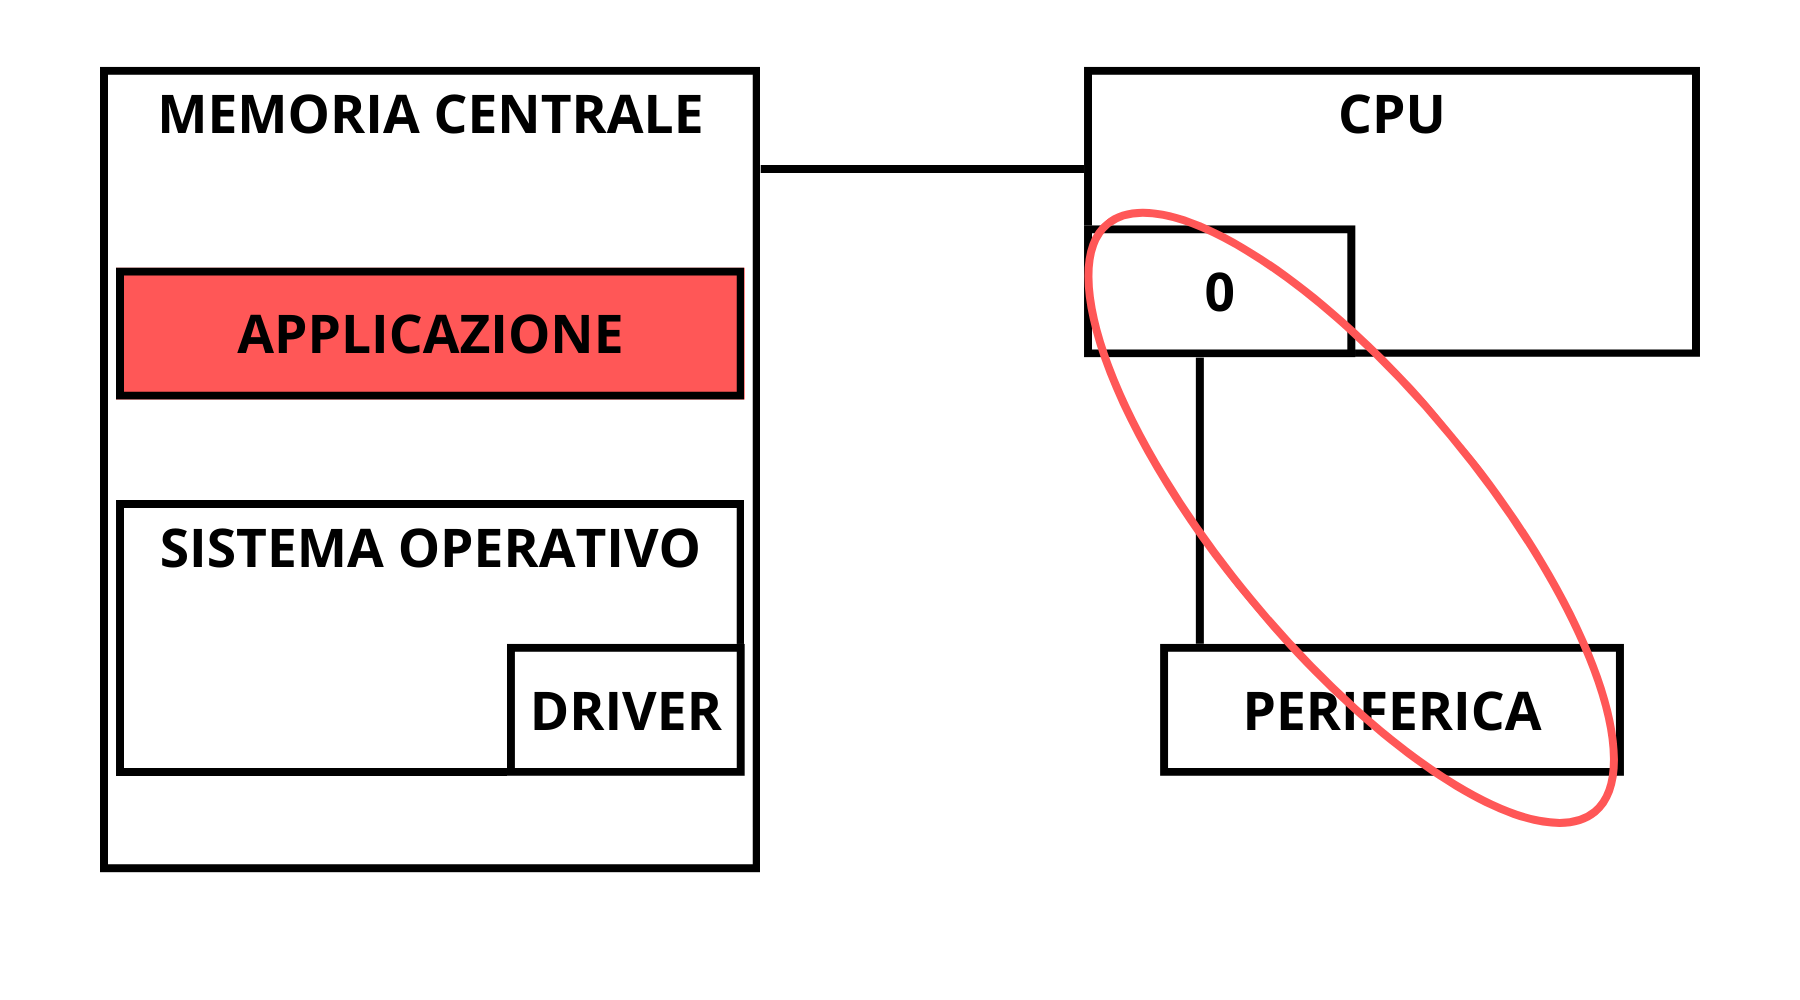
\includegraphics[width=\linewidth]{img/10.png}
        \caption{{creata con \href{https://www.canva.com/}{Canva}}}
    \end{figure}}
\end{frame}

\end{document}